\section{Introducción}

Este es un proyecto pequeño para probar GoLatex de punta a punta:
edición, compilación, errores parseados y sincronización en vivo
\citep{lamport1994latex}.
\begin{figure}[h]
  \centering
  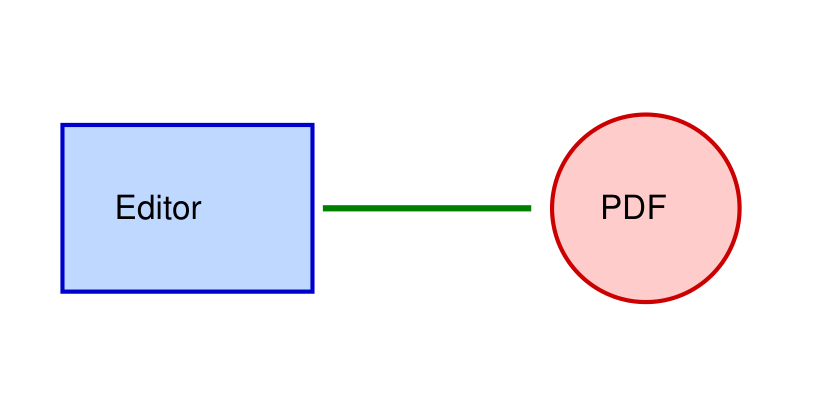
\includegraphics[width=0.7\linewidth]{img/diagrama.png}
  \caption{Un editor conectado a un PDF: la idea de GoLatex.}
  \label{fig:diagrama}
\end{figure}

Como muestra la Figura~\ref{fig:diagrama}, el flujo es directo. (Editado en vivo por el agente MCP.)
